%===============================================================================
% LaTeX sjabloon voor de bachelorproef toegepaste informatica aan HOGENT
% Meer info op https://github.com/HoGentTIN/latex-hogent-report
%===============================================================================

\documentclass[dutch,dit,thesis]{hogentreport}

% TODO:
% - If necessary, replace the option `dit`' with your own department!
%   Valid entries are dbo, dbt, dgz, dit, dlo, dog, dsa, soa
% - If you write your thesis in English (remark: only possible after getting
%   explicit approval!), remove the option "dutch," or replace with "english".

\usepackage{lipsum} % For blind text, can be removed after adding actual content

%% Pictures to include in the text can be put in the graphics/ folder
\graphicspath{{graphics/}}

%% For source code highlighting, requires pygments to be installed
%% Compile with the -shell-escape flag!
\usepackage[section]{minted}
%% If you compile with the make_thesis.{bat,sh} script, use the following
%% import instead:
%% \usepackage[section,outputdir=../output]{minted}
\usemintedstyle{solarized-light}
\definecolor{bg}{RGB}{253,246,227} %% Set the background color of the codeframe

%% Change this line to edit the line numbering style:
\renewcommand{\theFancyVerbLine}{\ttfamily\scriptsize\arabic{FancyVerbLine}}

%% Macro definition to load external java source files with \javacode{filename}:
\newmintedfile[javacode]{java}{
    bgcolor=bg,
    fontfamily=tt,
    linenos=true,
    numberblanklines=true,
    numbersep=5pt,
    gobble=0,
    framesep=2mm,
    funcnamehighlighting=true,
    tabsize=4,
    obeytabs=false,
    breaklines=true,
    mathescape=false
    samepage=false,
    showspaces=false,
    showtabs =false,
    texcl=false,
}

% Other packages not already included can be imported here

%%---------- Document metadata -------------------------------------------------
% TODO: Replace this with your own information
\author{Angela Degryse}
\supervisor{Sofie Lambert }
\cosupervisor{Tim Alenus}
\title%
    {State management in Flutter: een vergelijkende studie}
\academicyear{\advance\year by -1 \the\year--\advance\year by 1 \the\year}
\examperiod{1}
\degreesought{\IfLanguageName{dutch}{Professionele bachelor in de toegepaste informatica}{Bachelor of applied computer science}}
\partialthesis{false} %% To display 'in partial fulfilment'
\institution{The Mobility Factory}

%% Add global exceptions to the hyphenation here
\hyphenation{back-slash}

%% The bibliography (style and settings are  found in hogentthesis.cls)
\addbibresource{bachproef.bib}            %% Bibliography file
\addbibresource{../voorstel/voorstel.bib} %% Bibliography research proposal
\defbibheading{bibempty}{}

%% Prevent empty pages for right-handed chapter starts in twoside mode
\renewcommand{\cleardoublepage}{\clearpage}

\renewcommand{\arraystretch}{1.2}

%% Content starts here.
\begin{document}

%---------- Front matter -------------------------------------------------------

\frontmatter

\hypersetup{pageanchor=false} %% Disable page numbering references
%% Render a Dutch outer title page if the main language is English
\IfLanguageName{english}{%
    %% If necessary, information can be changed here
    \degreesought{Professionele Bachelor toegepaste informatica}%
    \begin{otherlanguage}{dutch}%
       \maketitle%
    \end{otherlanguage}%
}{}

%% Generates title page content
\maketitle
\hypersetup{pageanchor=true}

%%=============================================================================
%% Voorwoord
%%=============================================================================

\chapter*{\IfLanguageName{dutch}{Woord vooraf}{Preface}}%
\label{ch:voorwoord}

%% TODO:
%% Het voorwoord is het enige deel van de bachelorproef waar je vanuit je
%% eigen standpunt (``ik-vorm'') mag schrijven. Je kan hier bv. motiveren
%% waarom jij het onderwerp wil bespreken.
%% Vergeet ook niet te bedanken wie je geholpen/gesteund/... heeft

\lipsum[1-2]
%%=============================================================================
%% Samenvatting
%%=============================================================================

% TODO: De "abstract" of samenvatting is een kernachtige (~ 1 blz. voor een
% thesis) synthese van het document.
%
% Een goede abstract biedt een kernachtig antwoord op volgende vragen:
%
% 1. Waarover gaat de bachelorproef?
% 2. Waarom heb je er over geschreven?
% 3. Hoe heb je het onderzoek uitgevoerd?
% 4. Wat waren de resultaten? Wat blijkt uit je onderzoek?
% 5. Wat betekenen je resultaten? Wat is de relevantie voor het werkveld?
%
% Daarom bestaat een abstract uit volgende componenten:
%
% - inleiding + kaderen thema
% - probleemstelling
% - (centrale) onderzoeksvraag
% - onderzoeksdoelstelling
% - methodologie
% - resultaten (beperk tot de belangrijkste, relevant voor de onderzoeksvraag)
% - conclusies, aanbevelingen, beperkingen
%
% LET OP! Een samenvatting is GEEN voorwoord!

%%---------- Nederlandse samenvatting -----------------------------------------
%
% TODO: Als je je bachelorproef in het Engels schrijft, moet je eerst een
% Nederlandse samenvatting invoegen. Haal daarvoor onderstaande code uit
% commentaar.
% Wie zijn bachelorproef in het Nederlands schrijft, kan dit negeren, de inhoud
% wordt niet in het document ingevoegd.

\IfLanguageName{english}{%
\selectlanguage{dutch}
\chapter*{Samenvatting}
\lipsum[1-4]
\selectlanguage{english}
}{}

%%---------- Samenvatting -----------------------------------------------------
% De samenvatting in de hoofdtaal van het document

\chapter*{\IfLanguageName{dutch}{Samenvatting}{Abstract}}

\lipsum[1-4]


%---------- Inhoud, lijst figuren, ... -----------------------------------------

\tableofcontents

% In a list of figures, the complete caption will be included. To prevent this,
% ALWAYS add a short description in the caption!
%
%  \caption[short description]{elaborate description}
%
% If you do, only the short description will be used in the list of figures

\listoffigures

% If you included tables and/or source code listings, uncomment the appropriate
% lines.
%\listoftables
%\listoflistings

% Als je een lijst van afkortingen of termen wil toevoegen, dan hoort die
% hier thuis. Gebruik bijvoorbeeld de ``glossaries'' package.
% https://www.overleaf.com/learn/latex/Glossaries

%---------- Kern ---------------------------------------------------------------

\mainmatter{}

% De eerste hoofdstukken van een bachelorproef zijn meestal een inleiding op
% het onderwerp, literatuurstudie en verantwoording methodologie.
% Aarzel niet om een meer beschrijvende titel aan deze hoofdstukken te geven of
% om bijvoorbeeld de inleiding en/of stand van zaken over meerdere hoofdstukken
% te verspreiden!

%%=============================================================================
%% Inleiding
%%=============================================================================

\chapter{\IfLanguageName{dutch}{Inleiding}{Introduction}}%
\label{ch:inleiding}
Cross-platform ontwikkelen wordt steeds populairder omdat er vanuit één codebase de applicatie op meerdere toestellen gedraaid kan worden. Er bestaan veel cross-platform frameworks en Flutter is één van de bekendste die in 2018 door Google ontwikkeld werd. 



%De inleiding moet de lezer net genoeg informatie verschaffen om het onderwerp te begrijpen en in te zien waarom de onderzoeksvraag de moeite waard is om te onderzoeken. In de inleiding ga je literatuurverwijzingen beperken, zodat de tekst vlot leesbaar blijft. Je kan de inleiding verder onderverdelen in secties als dit de tekst verduidelijkt. Zaken die aan bod kunnen komen in de inleiding~\autocite{Pollefliet2011}:

%\begin{itemize}
%  \item context, achtergrond
 % \item afbakenen van het onderwerp
  %\item verantwoording van het onderwerp, methodologie
  %\item probleemstelling
  %\item onderzoeksdoelstelling
  %\item onderzoeksvraag
  %\item \ldots
%\end{itemize}

\section{\IfLanguageName{dutch}{Probleemstelling}{Problem Statement}}%
\label{sec:probleemstelling}
The Mobility Factory (TMF) is een coöperatie die IT-oplossingen biedt aan bedrijven die elektrische autodelen diensten aanbieden. De applicaties worden door de TMF-ontwikkelaars in Flutter geïmplementeerd. Omdat de applicaties van TMF steeds groter en complexer worden, werkt de applicatie steeds minder performant. Daarom kwam de vraag om de performantie van hun applicatie te optimaliseren. 

Een mogelijke reden van minder performante applicatie is door het slecht beheren van states. In Flutter zijn er tal van mogelijkheden voor het beheren van states. Afhankelijk van de complexiteit van de applicatie moet er overwogen worden welke state management benadering het best bij de applicatie past en of het de meest performante optie is.

\section{\IfLanguageName{dutch}{Onderzoeksvraag}{Research question}}%
\label{sec:onderzoeksvraag}

De hoofdonderzoekvraag van dit onderzoek is de volgende:
\\
\textbf{Op welk manier kan states bijgehouden worden in Flutter en welk past het bij bij de applicatie van The Mobility Factory?}
\\
\\
Daarnaast kan de hoofdonderzoekvraag verder verdeeld worden in de volgende deelonderzoeksvragen:
\begin{itemize}
  \item Welk benadering van state management is het performantste qua cpu-gebruik, opstartsnelheid, geheugengebruik...?
  \item Hoeveel moeite zal het The Mobility Factory kosten om de verschillende benaderingen van state management te implementeren? Hoe complex is het om te integreren in de bestaande code?
\end{itemize}

\section{\IfLanguageName{dutch}{Onderzoeksdoelstelling}{Research objective}}%
\label{sec:onderzoeksdoelstelling}

Het hoofddoel van dit onderzoek is om de developers van The Mobility Factory te helpen om een beslissing te maken of het veranderen van state management benadering een invloed kan hebben op de performantie van de applicatie. Ook zal er moeten overwogen worden of complexiteit om het te integreren in de bestaande code de moeite waard is. Dit wordt gedaan door middel van een vergelijkende studie. Eerst wordt er een literatuurstudie gedaan over de benaderingen van state management en daarna worden ze met elkaar vergeleken met behulp van een proof-of-concept.

\section{\IfLanguageName{dutch}{Opzet van deze bachelorproef}{Structure of this bachelor thesis}}%
\label{sec:opzet-bachelorproef}

% Het is gebruikelijk aan het einde van de inleiding een overzicht te
% geven van de opbouw van de rest van de tekst. Deze sectie bevat al een aanzet
% die je kan aanvullen/aanpassen in functie van je eigen tekst.

De rest van deze bachelorproef is als volgt opgebouwd:

In Hoofdstuk~\ref{ch:stand-van-zaken} wordt een overzicht gegeven van de stand van zaken binnen het onderzoeksdomein, op basis van een literatuurstudie.

In Hoofdstuk~\ref{ch:methodologie} wordt de methodologie toegelicht en worden de gebruikte onderzoekstechnieken besproken om een antwoord te kunnen formuleren op de onderzoeksvragen.

% TODO: Vul hier aan voor je eigen hoofstukken, één of twee zinnen per hoofdstuk

In Hoofdstuk~\ref{ch:conclusie}, tenslotte, wordt de conclusie gegeven en een antwoord geformuleerd op de onderzoeksvragen. Daarbij wordt ook een aanzet gegeven voor toekomstig onderzoek binnen dit domein.
\chapter{\IfLanguageName{dutch}{Stand van zaken}{State of the art}}%
\label{ch:stand-van-zaken}

In dit onderdeel wordt dieper ingegaan op wat flutter is hoe het werkt. Daarna wordt er onderzocht welke state management benaderingen er 
zijn en hoe ze werken en worden ze met elkaar vergeleken.

\section{{Flutter}}%
\label{sec:Flutter}
Flutter is een open-source framework ontwikkeld door Google coor het bouwen van multi-platform applicaties vanuit één codebase. 
Dit betekent dus dat ontwikkelaars in een korte tijd applicaties kunnen ontwikkelen voor mobiele, web, desktop en ook voor embedded systemen.
Bovendien wordt flutter code vertaald naar native machine code, wat zorgt voor snelle applicaties en annimaties. \footnote{\url{https://flutter.dev}}
\\
\\
Flutter applicaties worden geschreven met Dart, een programmeertaal die ook eigendom is van Google. Dart ondersteunt AOT (ahead of time) 
compilation en JIT (just in time) compilation. AOT verbetert de opstarttijd en performantie van de application en dankzij JIT compilation 
wordt hot reload mogelijk. Dit wilt zeggen dat enkel de gewijzigd stukken code opnieuw moet gecompileerd worden in plaats van de volledige applicatie.
Het is dus mogelijk om wijziginen in bijna real time te testen. \footnote{\url{https://docs.dart.dev}}

\section{Flutter Architectuur}
\label{sec:Flutter Architectuur}
Voor dat er over de state management binnen flutter besproken kan worden, wordt er eerst een paar begrippen uitgelegd binnen Flutter. Ook wordt er in dit deel
uitgelegd hoe Flutter werkt intern.

\subsection[widget]{Widgets}
\label{sec:Widgets}
In Flutter wordt alle componenten in de app als "Widget" beschouwd. Wat een widget is is eigenlijk een Dart klasse die beschrijft hoe een stuk van de user interface eruit ziet.
De UI van de app wordt dus met andere worden gebouwd door widgets in ouder-kind relatie te combineren. Elk widget wordt in een parent widget genest en context kan doorgegeven worden van ouder naar kind.
Alle widgets zitten dus in een widget boom, met elk ouder widget één of meerdere kind widgets.
\\
\begin{figure}[h]
    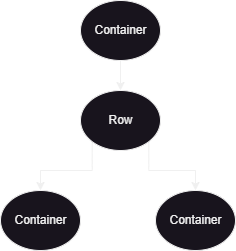
\includegraphics{graphics/widgetTree.png}
    \caption{Voorbeeld van een widget boom}
\end{figure}
\\
%TODO: add piece of code block for widget tree
Elk widget is onderanderlijk. Applicaties werken hun ui bij als reactie op gebeurtenissen (zoals een gebruikersinteractie) door het framework te vertellen 
dat een widet in de hiërarchie te vervangen door een andere widget. De ouder widgets worden met de nieuwe vergeleken door het framework en wordt de 
gebruikersinterface efficiënt bijgewerkt.


\subsection[states]{States}
\label{sec:States}
Elk widget kan states hebben. Flutter beschrijft een state als informatie die enerzijds synchroon kan worden gelezen wanneer de widget wordt gebouwd en anderzijds
kan veranderen tijdens de levensduur van de widget.  \footnote{\url{https://api.flutter.dev/flutter/widgets/State-class.html}}


\subsection[widget states]{Widget states}
\label{sec:Widget states}
Nu dat er een beeld is over wat states zijn binnen Flutter, kan er over de 2 meest gebruikte soorten widgets besproken worden. 
 \begin{itemize}
     \item stateless widget
     \item stateful widget
 \end{itemize}

\section{{State management}}%
\label{sec:State management}
Zoals eerder vermeld wordt Flutter ontwikkeld om performant te zijn. Maar een mogelijke reden die de performantie van de applicatie kan beïnvloeden is het slecht 
bijhouden van states binnen de applicatie.
\\
State management is een techniek, of meerdere, die gebruikt wordt om veranderingen in de applicatie te beheren. Het gebruik van de juiste state management kan zorgen 
voor betere leesbaarheid van code en ook voor een performanter applicatie. 
\subsection{{setState}}%
\label{sec:setState}
todo
\\
\subsection{{Provider}}%
\label{sec:Provider}
todo
\\
\subsection{{RiverPod}}%
\label{sec:RiverPod}
todo
\\
\subsection{{GetX}}%
\label{sec:GetX}
todo
\\
\subsection{{Redux}}%
\label{sec:Redux}
todo
\\
\subsection{{Bloc}}%
\label{sec:Bloc}
todo
\\
\subsection{{MobX}}%
\label{sec:MobX}
todo
% Tip: Begin elk hoofdstuk met een paragraaf inleiding die beschrijft hoe
% dit hoofdstuk past binnen het geheel van de bachelorproef. Geef in het
% bijzonder aan wat de link is met het vorige en volgende hoofdstuk.

% Pas na deze inleidende paragraaf komt de eerste sectiehoofding.

%Dit hoofdstuk bevat je literatuurstudie. De inhoud gaat verder op de inleiding, maar zal het onderwerp van de bachelorproef *diepgaand* uitspitten. De bedoeling is dat de lezer na lezing van dit hoofdstuk helemaal op de hoogte is van de huidige stand van zaken (state-of-the-art) in het onderzoeksdomein. Iemand die niet vertrouwd is met het onderwerp, weet nu voldoende om de rest van het verhaal te kunnen volgen, zonder dat die er nog andere informatie moet over opzoeken \autocite{Pollefliet2011}.

%Je verwijst bij elke bewering die je doet, vakterm die je introduceert, enz.\ naar je bronnen. In \LaTeX{} kan dat met het commando \texttt{$\backslash${textcite\{\}}} of \texttt{$\backslash${autocite\{\}}}. Als argument van het commando geef je de ``sleutel'' van een ``record'' in een bibliografische databank in het Bib\LaTeX{}-formaat (een tekstbestand). Als je expliciet naar de auteur verwijst in de zin (narratieve referentie), gebruik je \texttt{$\backslash${}textcite\{\}}. Soms is de auteursnaam niet expliciet een onderdeel van de zin, dan gebruik je \texttt{$\backslash${}autocite\{\}} (referentie tussen haakjes). Dit gebruik je bv.~bij een citaat, of om in het bijschrift van een overgenomen afbeelding, broncode, tabel, enz. te verwijzen naar de bron. In de volgende paragraaf een voorbeeld van elk.

%\textcite{Knuth1998} schreef een van de standaardwerken over sorteer- en zoekalgoritmen. Experten zijn het erover eens dat cloud computing een interessante opportuniteit vormen, zowel voor gebruikers als voor dienstverleners op vlak van informatietechnologie~\autocite{Creeger2009}.

%Let er ook op: het \texttt{cite}-commando voor de punt, dus binnen de zin. Je verwijst meteen naar een bron in de eerste zin die erop gebaseerd is, dus niet pas op het einde van een paragraaf.



%%=============================================================================
%% Methodologie
%%=============================================================================

\chapter{\IfLanguageName{dutch}{Methodologie}{Methodology}}%
\label{ch:methodologie}

%% TODO: In dit hoofstuk geef je een korte toelichting over hoe je te werk bent
%% gegaan. Verdeel je onderzoek in grote fasen, en licht in elke fase toe wat
%% de doelstelling was, welke deliverables daar uit gekomen zijn, en welke
%% onderzoeksmethoden je daarbij toegepast hebt. Verantwoord waarom je
%% op deze manier te werk gegaan bent.
%% 
%% Voorbeelden van zulke fasen zijn: literatuurstudie, opstellen van een
%% requirements-analyse, opstellen long-list (bij vergelijkende studie),
%% selectie van geschikte tools (bij vergelijkende studie, "short-list"),
%% opzetten testopstelling/PoC, uitvoeren testen en verzamelen
%% van resultaten, analyse van resultaten, ...
%%
%% !!!!! LET OP !!!!!
%%
%% Het is uitdrukkelijk NIET de bedoeling dat je het grootste deel van de corpus
%% van je bachelorproef in dit hoofstuk verwerkt! Dit hoofdstuk is eerder een
%% kort overzicht van je plan van aanpak.
%%
%% Maak voor elke fase (behalve het literatuuronderzoek) een NIEUW HOOFDSTUK aan
%% en geef het een gepaste titel.

\lipsum[21-25]



% Voeg hier je eigen hoofdstukken toe die de ``corpus'' van je bachelorproef
% vormen. De structuur en titels hangen af van je eigen onderzoek. Je kan bv.
% elke fase in je onderzoek in een apart hoofdstuk bespreken.

%\input{...}
%\input{...}
%...

%%=============================================================================
%% Conclusie
%%=============================================================================

\chapter{Conclusie}%
\label{ch:conclusie}

% TODO: Trek een duidelijke conclusie, in de vorm van een antwoord op de
% onderzoeksvra(a)g(en). Wat was jouw bijdrage aan het onderzoeksdomein en
% hoe biedt dit meerwaarde aan het vakgebied/doelgroep? 
% Reflecteer kritisch over het resultaat. In Engelse teksten wordt deze sectie
% ``Discussion'' genoemd. Had je deze uitkomst verwacht? Zijn er zaken die nog
% niet duidelijk zijn?
% Heeft het onderzoek geleid tot nieuwe vragen die uitnodigen tot verder 
%onderzoek?

\lipsum[76-80]



%---------- Bijlagen -----------------------------------------------------------

\appendix

\chapter{Onderzoeksvoorstel}

Het onderwerp van deze bachelorproef is gebaseerd op een onderzoeksvoorstel dat vooraf werd beoordeeld door de promotor. Dat voorstel is opgenomen in deze bijlage.

%% TODO: 
%\section*{Samenvatting}

% Kopieer en plak hier de samenvatting (abstract) van je onderzoeksvoorstel.

% Verwijzing naar het bestand met de inhoud van het onderzoeksvoorstel
%---------- Inleiding ---------------------------------------------------------

\section{Introductie}%
\label{sec:introductie}

Smartphones zijn een integraal onderdeel van ons dagelijks leven geworden. Daarom worden er steeds meer vraag om mobiele applicaties te ontwikkelen. Ook wordt cross-platform ontwikkelen steeds aantrekkelijker voor ontwikkelaars omdat ze in een kortere tijd applicaties kunnen ontwikkelen voor meerdere platformen.

The Mobility Factory (TMF) is een coöperatie die IT-oplossingen biedt aan bedrijven die elektrische autodelen diensten aanbieden. De applicaties worden door de TMF-ontwikkelaars in Flutter geïmplementeerd. Omdat de applicaties van TMF steeds groter en complexer worden, werkt de applicatie steeds minder performant. Daarom kwam de vraag om de performantie van hun applicatie te optimaliseren. 

In Flutter zijn er tal van mogelijkheden voor het beheren van states. Afhankelijk van de complexiteit van de applicatie moet er overwogen worden welke state management benadering het best bij de applicatie past en of het de meest performante optie is. In dit onderzoek wordt eerst de verschillende soorten state management benaderingen grondig besproken en daarna worden ze vergeleken met elkaar op basis van prestatie en code complexiteit aan de hand van een proof-of-concept. Hieruit wordt de onderzoeksvraag dus gecreëerd: \textit{Op welk manier kan states bijgehouden worden in Flutter en welk past het bij bij de applicatie van The Mobility Factory?}. De hoofdonderzoeksvraag kan verder verdeeld worden in de volgende deelonderzoeksvragen: 
\begin{itemize}
  \item Welk benadering van state management is het performantste qua cpu-gebruik, opstartsnelheid, geheugengebruik...?
  \item Hoeveel moeite zal het The Mobility Factory kosten om de verschillende benaderingen van state management te implementeren? Hoe complex is het om te integreren in de bestaande code?
\end{itemize}


%---------- Stand van zaken ---------------------------------------------------

\section{State-of-the-art}%
\label{sec:state-of-the-art}

Flutter is een open source raamwerk van Google voor het bouwen van  multi-platform applicaties vanuit één codebase, of met andere woorden een cross-platform raamwerk. Flutter werd in 2018 uitgebracht en wordt ondertussen door meer dan twee miljoen ontwikkelaars gebruikt om meer dan 350 duizend Flutter applicaties te ontwikkelen. \footnote{\url{https://flutter.dev/}}

\subsection{Application performance, een onderdeel van User Experience}
Applicatieperformantie is de werkelijke performantie die wordt ervaren door de eindgebruikers van de applicatie, zoals de gemiddelde responstijd bij normale belasting of piekbelasting \autocite{Rouse2014}.

Door een onderzoek van Google wordt er vastgesteld dat naarmate de laadsnelheid oploopt, hoe meer geneigd de gebruikers zijn om de website te verlaten \autocite{An2010}. Bij een laadsnelheid van meer dan 3 seconden van een webpagina, vertrekt 53\% van de gebruikers bij het inladen van de webpagina.

Volgens \textcite{Nielsen2010}, een UX-expert, is responsiviteit van een applicatie een basisregel voor het ontwerp van gebruikersinterfaces. De gebruikers moeten snel door de applicatie kunnen navigeren. Volgens Nielsen is een laadsnelheid tussen 1 en 10 seconden aanvaardbaar. Een laadsnelheid van langer dan 10 seconden kan ervoor zorgen dat de gebruiker afgeleid wordt waardoor het moeilijker is om geavanceerde taken tot een goed einde te brengen tegen dat de applicatie reageert.


\subsection{Technieken om applicatie performantie te verbeteren}
Flutter werd ontwikkeld om performant te zijn. Maar de prestatie van een Flutter applicatie kan sterk beïnvloed worden door hoe de applicatie ontworpen en geïmplementeerd wordt. \footnote{\url{https://docs.flutter.dev/perf/best-practices}}


Dit zijn 3 voorbeelden om de prestatie van een Flutter applicatie te verbeteren:
\begin{enumerate}
    \item \textbf{Memory management}
    \newline 
    Het memory management in Flutter wordt afgehandeld door de Dart Virtual Machine (DVM), die een garbage collector heeft die automatisch ongebruikte geheugen terughaalt. Er kunnen echter nog steeds geheugenlekken optreden als objecten niet op de juiste manier uit het geheugen worden vrijgegeven, waardoor ze in de heap blijven hangen en onnodige bronnen verbruiken. Om geheugenlekken te vermijden moet de Dispose-methode gebruikt worden om onnodige objecten te verwijderen. \autocite{sabbagh2023}
    \item \textbf{Netwerk optimalisatie}
    \newline 
    Om netwerk prestatie te verhogen moet er gebruik gemaakt worden van efficiënte netwerk libraries zoals Dio. Ook door de gegevens te cachen op het apparaat van de gebruiker kan er onnodige netwerkverzoeken vermeden worden en wordt de latentie verminderd. \footnote{\url{https://www.linkedin.com/pulse/flutter-performance-optimization-techniques-best-practices/}}
    \item \textbf{State management}
    \newline Binnen dit onderzoek wordt er gefocust op dit onderdeel. Dit wordt verder beschreven in het volgende puntje \hyperref[sec:states]{2.4}
\end{enumerate}

\subsection{State management binnen Flutter}
\label{sec:states}
Flutter beschrijft een state als informatie die enerzijds synchroon kan worden gelezen wanneer de widget wordt gebouwd en anderzijds kan veranderen tijdens de levensduur van de widget. \footnote{\url{https://api.flutter.dev/flutter/widgets/State-class.html}}
\newline
States worden niet van parent widget naar child widget doorgegeven. De state van een widget wordt beheerd door zichzelf of door een parent widget en als de state van de parent widget wijzigt, moet alle widgets onder die parent widget ook herladen worden. Daarom kan het apart beheren van states zorgen voor efficiëntere updates en betere prestaties van de applicatie, aangezien enkel betreffende widgets heropgebouwd moeten worden. Deze functie is vooral gunstig voor complexe applicaties, waar het herbouwen van de volledige widgetstructuur tijdrovend kan zijn en kan leiden tot ondermaatse prestaties. Het is dus van groot belang dat de juiste benadering van state management wordt toegepast, zodat het optimaal presteert en een naadloze gebruikerservaring garandeert. \autocite{sid2023}

Dit zijn de mogelijke benaderingen van state management in Flutter: 
\begin{itemize}
    \item SetState
    \item Provider
    \item GetX
    \item RiverPod
    \item Redux
    \item BLoC / Rx
    \item MobX
\end{itemize}

\subsection{Relevante studies}
State management wordt door het Flutter-team als complex bestempeld en er wordt veel gediscussieerd onder de Flutter-ontwikkelaars over wat de beste aanpak is.

Een vergelijkbaar onderzoek dat reeds werd gedaan over state management is door \textcite{Vriest2019}. Hoewel zijn onderzoek maar 3 jaar oud is, is Flutter heel sterk geëvolueerd sindsdien. Zijn onderzoek concludeerde dat Provider het meest performant is voor een simpel CRUD-applicatie. Maar in zijn onderzoek waren er tekortkomingen, zoals het enkel testen op een Android-toestel en ook werden data niet van een API opgehaald, wat niet realistisch is voor de realiteit.

 Een andere vergelijkbaar onderzoek werd door \textcite{slep2020} geschreven. In zijn onderzoek werd de verschillende benaderingen van state management gegroepeerd en vergeleken. In zijn onderzoek werden er criteria opgesteld om het best passende benadering te kiezen voor de verschillende use cases.


%---------- Methodologie ------------------------------------------------------
\section{Methodologie}%
\label{sec:methodologie}

Eerst zal een vergelijkende studie uitgevoerd worden door de verschillende benaderingen van state management op te sommen en hun voor- en nadelen te vergelijken. Uit de gevonden state management benaderingen zullen er vier uitgekozen worden om toe te passen in het proof-of-concept.


In het methodologiegedeelte zullen verschillende versies van een bepaalde feature van de applicatie van TMF geïmplementeerd worden, waarbij voor elke versie een andere benadering van state management wordt toegepast. De applicatie van TMF die nagemaakt zal worden is een beheerapplicatie om reservaties en gebruikers te beheren.

De prestaties van de applicatie zullen getest worden op basis van CPU-gebruik, laadsnelheid en nodige opslag voor de applicatie. Er wordt ook een afweging gemaakt tussen de prestaties die worden geleverd door state management en de complexiteit van de integratie ervan in de bestaande code.

Het proof-of-concept zal geïmplementeerd worden met Flutter op Visual Studio Code. De applicatie van TMF wordt voornamelijk gebruikt op de web, daarom zal de performantie van de proof-of-concept getest worden als een webapplicatie en ook op een fysieke iOS-toestel. De code complexiteit van de state managements zullen vergeleken worden op basis van aantal nodige lijnen code. 
Om de performantie te meten zal er automated integration testen geschreven en uitgevoerd worden aan de hand van Flutter Driver. Bij elk uitvoering van de testen zullen de performantie gemeten worden. \footnote{\url{https://docs.flutter.dev/cookbook/testing/integration/profiling}}



%---------- Verwachte resultaten ----------------------------------------------
\section{Verwachte resultaten}%


\label{sec:verwachte-resultaten}
Uit eerdere onderzoeken blijkt dat Provider het best benadering van state management is op vlak van complexiteit en ook op prestatie vlak. Dit is ook de state management benadering die aanbevolen wordt door Flutter. Maar omdat de applicatie van TMF complexer is, wordt er verwacht dat Bloc een betere benadering van state management zal zijn.


\section{Discussie, conclusie}%
\label{sec:discussie-conclusie}
Er zijn talloze manieren om de prestaties van een Flutter-applicatie te verhogen. Een van de manieren is om het meest geschikte state management toe te passen, afhankelijk van de complexiteit van de geïmplementeerde applicatie. 

Het doel van deze studie is om TMF-ontwikkelaars een idee te geven van welke state management opties beschikbaar zijn in Flutter en wat het meest performant is voor hun applicatie. 




%%---------- Andere bijlagen --------------------------------------------------
% TODO: Voeg hier eventuele andere bijlagen toe. Bv. als je deze BP voor de
% tweede keer indient, een overzicht van de verbeteringen t.o.v. het origineel.
%\input{...}

%%---------- Backmatter, referentielijst ---------------------------------------

\backmatter{}

\setlength\bibitemsep{2pt} %% Add Some space between the bibliograpy entries
\printbibliography[heading=bibintoc]

\end{document}
